\chapter{Referencial Teórico}\label{cap:referencial_teorico}

\section{Twitter}\label{sec:twitter}

Contando com uma base ativa de usuários que ultrapassa 300 milhões\cite{twittercompany2016}, o Twitter é conhecido como um \emph{microblog} fundado em março de 2006 por Jack Dorsey, Evan Williams e Biz Stone. Após 10 anos de mercado, a empresa acumula números impressionantes: 300 bilhões de mensagens já foram compartilhadas por seus usuários, que em média enviam 500 milhões de \emph{tweets}\cite{twitterstats2016} - nome pelo qual as mensagens ficaram conhecidas na internet - por dia. Os usuários trocam mensagens de até 140 caracteres\cite{twittercharlimit2016} em um ambiente de rede social, que tem como objetivo dar à todos o poder de criar e compartilhar ideias e informações instantaneamente, sem barreiras\cite{twittercompany2016}. 

Dentro do Twitter, O usuário pode fazer uso de marcadores conhecidos como \emph{hashtags}\cite{waite2012paperback}, para vincular sua mensagem à um tópico específico. Apesar de simples, as \emph{hashtags} pode ser usadas das mais diversas maneiras:
\begin{itemize}
\item Agrupar comentários e pensamentos acerca de um tema
\item Estabelecer uma conexão entre dois tópicos
\item Aproximar o usuários de um conteúdo relevante com auxílio de uma busca
\end{itemize}

Um dos exemplos mais recentes e impressionantes de como as redes sociais desempenharam o papel de aproximar ideologias semelhantes e encorajar debates profundos foi a Primavera Árabe - onda de manifestações e protestos que tiveram início em dezembro de 2010, tendo como cenário o Norte da África e Oriente Médio. Os principais alvos foram os regimes ditatoriais e patriarcais que há muito tempo estavam no poder.\cite{howard2011opening}. Através de discussões sobre democracia e direitos democráticos, protestos, manifestações e guerras civis foram tr

Este novo cenário possibilitou que a análise de redes sociais ganhasse incrível relevância nos campos de pesquisa social e comportamental\cite{wasserman1994advances}. A facilidade de acesso, o grande volume de dados, além da observação dos atores sociais e suas interações abre novas perspectivas dentro da pesquisa social e comportamental a cada dia.

\section{Mineração de opinião}\label{sec:mineracao_dados}

* O que é?* Exemplos no mercado* Etapas(http://www.inf.ufsc.br/~alvares/INE5644/MineracaoOpiniao.pdf)

É de conhecimento comum que há um acúmulo de dados por toda a internet. Artigos, informações de usuários, comportamento de usuários, essas são alguns tipos de informação que pode ser encontrada hoje na internet. Esse grande acumulo não garante informações confiáveis ou uma análise correta sobre os dados, por isso hoje há uma grande urgência para novas teorias computacionais e ferramentas que ajudem a analisar essa quantidade de dados que só aumenta \cite{fayyad1996data}. E dentro dessa enorme gama de dados, existem as informações adicionadas por usuários através de texto que remetem a suas reações a determinadas situações ou objetos.

\begin{figure}[ht]
	
	\centering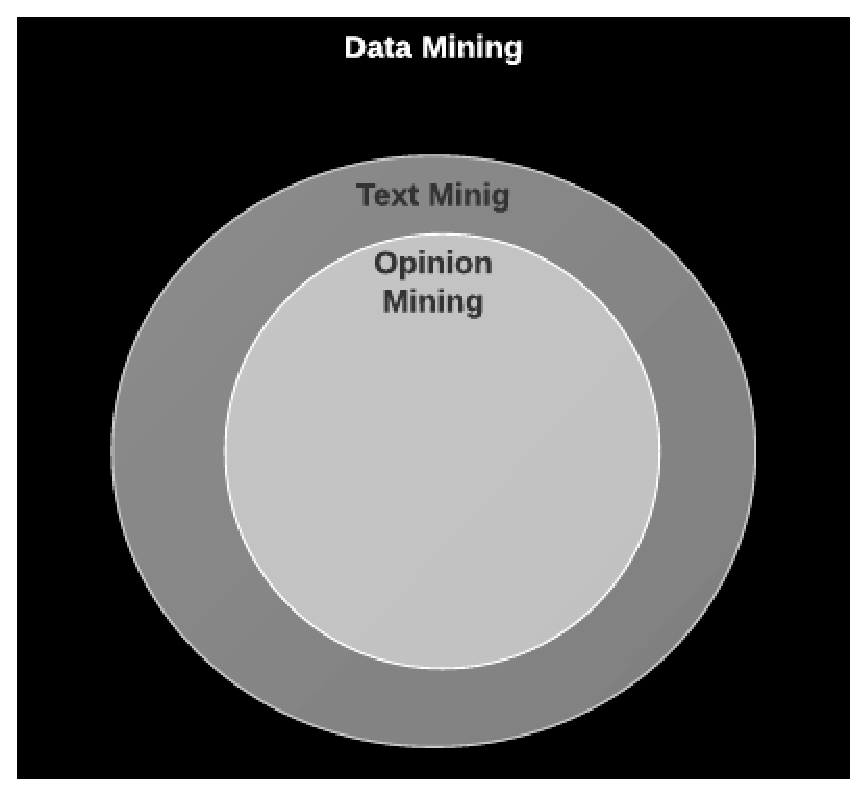
\epsfig{file=figuras/venn.eps, width=5cm}
	\caption{Diagrama de Venn - Mineração de Dados}
	\label{uni}
\end{figure}

A mineração de opinião também conhecida como mineração de sentimento, análise de sentimento ou extração de opinião, é um campo dentro da mineração de dados \cite{santos2014mineraccao}. Ela tem como intuito extrair o sentimento do texto escrito por uma pessoa, mas fazendo isso sem a interferência humana. Existe  dificuldade em afirmar o que é sentimento, na maioria dos dicionários sentimento é:
\begin{itemize}
\item Ato ou efeito de sentir.
\item Aptidão para receber as impressões.
\item Sensação; sensibilidade.
\item Consciência íntima.
\item Faculdade de compreender; intuição; percepção.
\end{itemize}

Porém de acordo com psicólogo Klaus R. Scherer em \cite{scherer2001emotional}, sentimento é um breve episódio da resposta sincronizada de todos os ou grande parte dos subsistemas orgânicos em resposta a um evento interno ou externo de grande significância.

 

\section{API}\label{sec:api}
* O que é
* APIs mais utilizadas no mundo (case do twitter)
* Papel de uma API para integração de serviços (achar referência foda)

\section{Processamento de linguagem natural}\label{sec:nlp}
* Linguagem natural (foto da matéria de autômato do Aquino?)
* Processamento de linguagem natural
* Dificuldades dentro da nossa área de estudo


\section{Naive Bayes}\label{sec:naive_bayes}
* O que é o Naive Bayes
* Demonstração matemática do algoritmo
* Uso dele em analise de sentimento/classificação


\emph{Naive Bayes} é um algoritmo probabilístico. Baseado no teorema de bayes. $$ P(A \mid B) = \frac{P(B \mid A) \, P(A)}{P(B)} $$ onde se infere qual é a probabilidade de um evento A dado um evento B. Porém nesse trabalho é utilizado o \emph{Naive Bayes} e sua diferença para o teorema de Bayes é assumir que a posição das palavras que aparecem no texto não importa, daí é acrescentado o \emph{naive}(ingênuo) ao teorema.
\\ Como visto em \cite{lucca2013implementaccao} o algoritmo computa qual a probabilidade de uma frase, denominada de documento pertencer a uma determinada classe(polaridade) \emph{P(c/d)}, a partir da probabilidade a \emph{priori} de \emph{P(c)} do documento pertencer a esta classe e da probabilidades condicionais de cada termo \emph{tk} ocorrer em um documento da mesma classe. O algoritmo tem como objetivo encontrar a melhor classe para um documento maximizando a probabilidade a\emph{posteriori} conforme a equação abaixo, onde $ n_{d} $ é o número de termos no documento \emph{d}. $$ C_{map}= argmax_{c \epsilon C}P(c|d)=argmax_{c \epsilon C}P(c)\prod 1sksn_{d}P(t_{k}/d) $$